\documentclass[11pt]{article}
\newcommand{\ArticleShortTitle}{Аудируемая оценка BVC}
\newcommand{\ArticlePDFTitle}{Аудируемая оценка многоролевых LLM-алгоритмов на реальных программных задачах}
\usepackage[a4paper,top=22mm,bottom=22mm,left=22mm,right=22mm,headheight=22pt]{geometry}
\usepackage{fontspec}
\defaultfontfeatures{Ligatures=TeX,Scale=MatchLowercase}
\setmainfont{times.ttf}[
  Path=C:/Windows/Fonts/,
  BoldFont=timesbd.ttf,
  ItalicFont=timesi.ttf,
  BoldItalicFont=timesbi.ttf
]
\setsansfont{arial.ttf}[
  Path=C:/Windows/Fonts/,
  BoldFont=arialbd.ttf,
  ItalicFont=ariali.ttf,
  BoldItalicFont=arialbi.ttf
]
\setmonofont{consola.ttf}[
  Path=C:/Windows/Fonts/,
  BoldFont=consolab.ttf,
  ItalicFont=consolai.ttf,
  BoldItalicFont=consolaz.ttf,
  Scale=0.82
]
\usepackage[main=russian,english]{babel}
\usepackage{microtype}

\usepackage{amsmath,amssymb,mathtools}
\usepackage{booktabs,tabularx,array,longtable,multirow}
\usepackage{graphicx}
\graphicspath{{figures/}}
\usepackage{float}
\usepackage[section]{placeins}
\usepackage{caption}
\usepackage{subcaption}
\usepackage{enumitem}
\usepackage{siunitx}
\sisetup{
  output-decimal-marker={,},
  group-separator={\,},
  group-minimum-digits=4,
  detect-all
}
\usepackage{xcolor}
\definecolor{Ink}{HTML}{0F172A}
\definecolor{Muted}{HTML}{475569}
\definecolor{Rule}{HTML}{CBD5E1}
\definecolor{BVC}{HTML}{7C3AED}
\definecolor{Cyan}{HTML}{0EA5E9}
\definecolor{Teal}{HTML}{14B8A6}
\definecolor{Amber}{HTML}{F59E0B}
\definecolor{Soft}{HTML}{F8FAFC}
\usepackage[most]{tcolorbox}
\newtcolorbox{resultbox}[1][]{
  enhanced,
  breakable,
  colback=Soft,
  colframe=BVC,
  boxrule=0.8pt,
  arc=1.5mm,
  left=3mm,right=3mm,top=2mm,bottom=2mm,
  title={#1},
  fonttitle=\bfseries\sffamily,
  coltitle=Ink
}
\newtcolorbox{methodbox}[1][]{
  enhanced,
  breakable,
  colback=white,
  colframe=Rule,
  boxrule=0.6pt,
  arc=1.5mm,
  left=3mm,right=3mm,top=2mm,bottom=2mm,
  title={#1},
  fonttitle=\bfseries\sffamily,
  coltitle=Ink
}

\usepackage{tikz}
\usetikzlibrary{arrows.meta,positioning,shapes.geometric,calc,fit}
\tikzset{
  stage/.style={draw=Rule,rounded corners=2mm,fill=Soft,minimum height=11mm,
    text width=28mm,align=center,font=\small\sffamily},
  gate/.style={diamond,draw=BVC,fill=BVC!7,aspect=1.8,align=center,
    inner sep=1.2mm,font=\small\sffamily},
  flow/.style={-{Latex[length=2.2mm]},thick,draw=Muted},
  note/.style={font=\scriptsize\sffamily,text=Muted,align=center}
}

\usepackage{titlesec}
\titleformat{\section}{\Large\bfseries\sffamily\color{Ink}}{\thesection.}{0.55em}{}
\titleformat{\subsection}{\large\bfseries\sffamily\color{Ink}}{\thesubsection.}{0.55em}{}
\titleformat{\subsubsection}{\normalsize\bfseries\sffamily\color{Ink}}{\thesubsubsection.}{0.55em}{}
\titlespacing*{\section}{0pt}{2.2ex plus .5ex minus .2ex}{1.0ex}
\titlespacing*{\subsection}{0pt}{1.8ex plus .4ex minus .2ex}{0.8ex}

\usepackage{fancyhdr}
\pagestyle{fancy}
\fancyhf{}
\fancyhead[L]{\small\sffamily\color{Muted}\ArticleShortTitle}
\fancyhead[R]{\small\sffamily\color{Muted}Xynapse / BVC}
\fancyfoot[C]{\small\sffamily\color{Muted}\thepage}
\renewcommand{\headrulewidth}{0.4pt}
\renewcommand{\headrule}{\hbox to\headwidth{\color{Rule}\leaders\hrule height \headrulewidth\hfill}}

\usepackage{csquotes}
\usepackage[
  backend=biber,
  style=numeric-comp,
  sorting=nyt,
  maxbibnames=8,
  giveninits=true,
  doi=true,
  url=true,
  isbn=false
]{biblatex}
\addbibresource{references.bib}
\AtBeginBibliography{\footnotesize\sloppy\hbadness=10000\relax}

\usepackage{hyperref}
\hypersetup{
  colorlinks=true,
  linkcolor=BVC,
  citecolor=BVC,
  urlcolor=Cyan,
  pdftitle={\ArticlePDFTitle},
  pdfauthor={Халилов Джабраиль Эльнурович},
  pdfsubject={Экспериментальная оценка BVC},
  pdfkeywords={BVC, SWE-bench Verified, LLM, программирование, Xynapse}
}
\usepackage[nameinlink,noabbrev]{cleveref}

\captionsetup{
  font=small,
  labelfont={bf,sf,color=Ink},
  textfont={color=Muted},
  justification=centering,
  singlelinecheck=false,
  skip=5pt
}
\setlist[itemize]{leftmargin=1.5em,itemsep=0.25em,topsep=0.35em}
\setlist[enumerate]{leftmargin=1.6em,itemsep=0.25em,topsep=0.35em}
\renewcommand{\arraystretch}{1.15}
\setlength{\tabcolsep}{5pt}
\setlength{\parindent}{1.15em}
\setlength{\parskip}{0.18em}
\setlength{\emergencystretch}{4em}
\tolerance=1200

\newcommand{\BVCname}{Bounded Verification Council (BVC)}
\newcommand{\pp}{п.\,п.}
\newcommand{\dataset}{SWE-bench Verified}
\newcommand{\code}[1]{\texttt{#1}}
\newcommand{\sourcehash}[1]{\texttt{\footnotesize #1}}

% Auto-generated by generate_analysis_assets.py. Do not edit by hand.
\newcommand{\NTasks}{60}
\newcommand{\NRepos}{11}
\newcommand{\NPrimaryRuns}{240}
\newcommand{\NRepeatRuns}{90}
\newcommand{\NVibeRuns}{45}
\newcommand{\NAllRuns}{375}
\newcommand{\DirectResolved}{4}
\newcommand{\SingleResolved}{7}
\newcommand{\BVCResolved}{5}
\newcommand{\FixedResolved}{6}
\newcommand{\DirectRate}{6.7}
\newcommand{\SingleRate}{11.7}
\newcommand{\BVCRate}{8.3}
\newcommand{\FixedRate}{10.0}
\newcommand{\DirectWilsonLow}{2.6}
\newcommand{\DirectWilsonHigh}{15.9}
\newcommand{\SingleWilsonLow}{5.8}
\newcommand{\SingleWilsonHigh}{22.2}
\newcommand{\BVCWilsonLow}{3.6}
\newcommand{\BVCWilsonHigh}{18.1}
\newcommand{\FixedWilsonLow}{4.7}
\newcommand{\FixedWilsonHigh}{20.1}
\newcommand{\BVCCalls}{472}
\newcommand{\FixedCalls}{600}
\newcommand{\DirectCalls}{60}
\newcommand{\SingleCalls}{120}
\newcommand{\BVCTokens}{14282809}
\newcommand{\FixedTokens}{18365172}
\newcommand{\DirectTokens}{1867093}
\newcommand{\SingleTokens}{3585838}
\newcommand{\BVCCost}{1838.46}
\newcommand{\FixedCost}{2402.61}
\newcommand{\DirectCost}{312.44}
\newcommand{\SingleCost}{522.84}
\newcommand{\BVCCostTask}{30.64}
\newcommand{\FixedCostTask}{40.04}
\newcommand{\DirectCostTask}{5.21}
\newcommand{\SingleCostTask}{8.71}
\newcommand{\BVCCostResolved}{367.69}
\newcommand{\FixedCostResolved}{400.44}
\newcommand{\DirectCostResolved}{78.11}
\newcommand{\SingleCostResolved}{74.69}
\newcommand{\CallsSaved}{128}
\newcommand{\CallsSavedPct}{21.3}
\newcommand{\TokensSaved}{4082363}
\newcommand{\TokensSavedPct}{22.2}
\newcommand{\CostSaved}{564.15}
\newcommand{\CostSavedPct}{23.5}
\newcommand{\CostResolvedSavedPct}{8.2}
\newcommand{\TokensSavedTask}{68039}
\newcommand{\CostSavedTask}{9.40}
\newcommand{\CallsSavedTaskMean}{2.13}
\newcommand{\CallsSavedTaskMeanLow}{1.60}
\newcommand{\CallsSavedTaskMeanHigh}{2.67}
\newcommand{\CallsSavedTaskMedian}{4}
\newcommand{\TokensSavedTaskMeanLow}{51980}
\newcommand{\TokensSavedTaskMeanHigh}{83480}
\newcommand{\TokensSavedTaskMedian}{111910}
\newcommand{\CostSavedTaskMeanLow}{6.75}
\newcommand{\CostSavedTaskMeanHigh}{12.05}
\newcommand{\CostSavedTaskMedian}{7.92}
\newcommand{\TokensOverrunTasks}{11}
\newcommand{\TokensOverrunMax}{13971}
\newcommand{\CostOverrunTasks}{10}
\newcommand{\CostOverrunMax}{12.84}
\newcommand{\BVCShort}{32}
\newcommand{\BVCExtended}{28}
\newcommand{\BVCShortResolved}{5}
\newcommand{\BVCExtendedResolved}{0}
\newcommand{\BVCShortTokensMean}{179160}
\newcommand{\BVCExtendedTokensMean}{305345}
\newcommand{\BVCShortCostMean}{22.78}
\newcommand{\BVCExtendedCostMean}{39.62}
\newcommand{\FixedShortResolved}{5}
\newcommand{\FixedExtendedResolved}{1}
\newcommand{\GateUndefinedVote}{7}
\newcommand{\GateFourValidAxes}{35}
\newcommand{\GateThreeValidAxes}{18}
\newcommand{\GateZeroValidAxes}{7}
\newcommand{\GateMetricCorrelation}{0.412}
\newcommand{\AllTokens}{54533372}
\newcommand{\AllCost}{7266.84}
\newcommand{\CostCap}{11800}



\title{\vspace{-1.2em}\textbf{\sffamily Аудируемая оценка многоролевых LLM-алгоритмов\\
на реальных программных задачах}}
\author{Халилов Джабраиль Эльнурович\\
\small Национальный исследовательский университет «Высшая школа экономики»\\
\small Исследовательский проект Xynapse / BVC\\
\small \href{https://github.com/jabrailkhalil/xynapse}{\nolinkurl{github.com/jabrailkhalil/xynapse}}}
\date{2026}

\begin{document}
\maketitle

\begin{abstract}
Полезный LLM-алгоритм должен быть не только запущен, но и проверяем: каждое
утверждение о качестве и стоимости должно восстанавливаться до конкретной
задачи, prompt, patch и результата тестов. Такая оценка требует контролировать
выбор задач, кодовый контекст, версию модели, полноту генерации, исполняемое
тестирование и статистический анализ парных исходов. В статье описан
аудируемый контур проверки Bounded Verification Council (BVC), созданный
как экспериментальное продолжение дипломного проекта Xynapse. Основная
матрица содержит \NPrimaryRuns{} запусков: четыре метода на одних и тех же
\NTasks{} задачах \dataset{}. Дополнительно выполнены \NRepeatRuns{}
строк аудита повторяемости и \NVibeRuns{} запусков с разговорной
формулировкой; общий объём официальной оценки равен \NAllRuns{} строкам.
Все ожидаемые финальные результаты присутствуют, дубликаты отсутствуют,
несовпадения hash prompt и content равны нулю. Для сравнения качества
использованы парная разность долей, точный критерий Мак-Немара и
стратифицированный paired bootstrap на 10\,000 выборок. BVC решил 5/60
задач, один предварительный план --- 7/60, direct --- 4/60, полный совет
--- 6/60. Основное сравнение BVC с одним планом дало \(-3{,}3\)
процентного пункта, 95\% интервал \([-10{,}0;+3{,}3]\), \(p=0{,}625\).
Следовательно, гипотеза преимущества качества не подтверждена; одновременно
нижняя граница интервала лежит ниже заранее заданного margin \(-5\) \pp,
поэтому неухудшаемость также не установлена. Практическая ценность контура
состоит в том, что он превращает BVC из демонстрации идеи в измеримый
инженерный объект и проверяемо разделяет статистический вывод, описательный
сигнал и ресурсную эффективность.
\end{abstract}

\noindent\textbf{Ключевые слова:} аудируемость, воспроизводимость, LLM-агенты,
программная инженерия, \dataset{}, парный эксперимент, bootstrap,
критерий Мак-Немара, Xynapse, BVC.

\section{Введение}

Бинарный ответ \enquote{patch прошёл тесты} кажется простой метрикой, однако
путь к достоверному сравнению методов состоит из многих зависимых решений.
Если методы видят разные файлы, задача перестаёт быть парной. Если задачи
выбраны после просмотра outcome, оценка становится оптимистичной. Если
провайдерский timeout удаляется как \enquote{неудачный запуск}, нарушается
полнота. Если методы сравниваются только по агрегированным процентам,
игнорируется тот факт, что они решали одни и те же instances.

В выпускной квалификационной работе автора описана интеллектуальная среда
Xynapse с интегрированным AI-ассистентом и многоролевым механизмом
планирования \cite{khalilov2026}. Для переноса проектной идеи в научное
утверждение потребовался отдельный контур, в котором алгоритм, данные и
правила вывода фиксируются до наблюдения результата. Настоящая статья
описывает именно этот контур. Программный проект Xynapse и его актуальная
реализация доступны в открытом репозитории \cite{xynapse2026}; диплом
цитируется как источник архитектуры, а репозиторий --- как источник кода.

В отличие от демонстрации отдельных удачных patch, исследование использует
реальные задачи \dataset{} \cite{jimenez2024swebench}, одинаковый исходный
контекст, четыре заранее определённых метода и официальный исполняемый
evaluator. Результат каждого этапа сохраняется как машиночитаемый артефакт
с SHA-256. Такая структура позволяет заново построить сводные таблицы и
графики из исходных JSONL, не доверяя вручную переписанным значениям.

\begin{resultbox}[Основные принципы контура]
\begin{itemize}
  \item outcome-blind выборка и замороженный протокол;
  \item одинаковая задача, кодовый контекст и финальная patch-инструкция;
  \item task-level pairing между методами;
  \item сохранение невалидных и неуспешных результатов без post-hoc удаления;
  \item официальный запуск тестов, а не экспертная оценка правдоподобия;
  \item отдельные серии для повторяемости и разговорной формулировки;
  \item хэшируемая цепочка от матрицы генерации до итогового анализа.
\end{itemize}
\end{resultbox}

\begin{resultbox}[Что этот контур даёт инженерной команде]
\begin{itemize}
  \item любой итоговый процент можно проследить до конкретной задачи, ответа,
        patch и официального теста;
  \item неуспехи и инфраструктурные случаи остаются видимыми, поэтому удачные
        примеры нельзя незаметно отбирать post hoc;
  \item качество и расход ресурсов анализируются раздельно, что позволяет
        честно использовать доказанную экономию без завышения claims;
  \item модель, выборку или тариф можно заменить, сохранив дизайн сравнения и
        повторно рассчитав агрегаты из машиночитаемых артефактов.
\end{itemize}
Это делает экспериментальный контур самостоятельным результатом: он пригоден
не для одной презентации, а для последовательного развития BVC.
\end{resultbox}

\section{Исследовательские вопросы}

Контур отвечает на четыре разных вопроса.

\begin{enumerate}
  \item \textbf{Качество.} Решает ли BVC больше задач, чем один
        предварительный план? Это первичный contrast.
  \item \textbf{Дополнительные ориентиры.} Как BVC соотносится с direct и
        полным советом?
  \item \textbf{Эффективность.} Какой фактический расход вызовов, токенов и
        расчётной стоимости несёт каждый метод?
  \item \textbf{Устойчивость.} Насколько бинарный outcome повторяется при
        temperature \(=0\) и сохраняется при переходе от формальной к
        разговорной постановке?
\end{enumerate}

Разделение важно: положительная ресурсная метрика не превращается
автоматически в утверждение о качестве, а единичное превышение процента
успехов не объявляется доказанным преимуществом.

\section{Данные и outcome-blind выборка}

\subsection{Источник задач}

\dataset{} представляет программную задачу как реальное issue и состояние
репозитория, к которому модель должна построить применимый patch
\cite{jimenez2024swebench}. Версия Verified была сформирована как 500
примеров после независимой проверки каждой задачи тремя разработчиками и
отсечения серьёзно недоопределённых условий или некорректных тестов
\cite{openai2024verified}. Из зафиксированной ревизии набора
\code{91aa3ed51b709be6457e12d00300a6a596d4c6a3} выбрано 60 instances.
Выборка сформирована до генерации итоговых patch.

\begin{table}[H]
\centering
\caption{Стратификация 60 задач по оценке трудоёмкости.}
\label{tab:strata}
\begin{tabular}{@{}lrr@{}}
\toprule
Страта & Число задач & Доля\\
\midrule
Medium: 15 минут--1 час & 30 & 50,0\%\\
Hard: 1--4 часа & 27 & 45,0\%\\
Very hard: более 4 часов & 3 & 5,0\%\\
\bottomrule
\end{tabular}
\end{table}

Задачи происходят из 11 Python-репозиториев. Наличие нескольких проектов
уменьшает зависимость результата от одной кодовой базы, хотя выборка не
предназначена для точной оценки каждого репозитория отдельно.

Отбор был полностью алгоритмическим. Взяты все 3 задачи \(>4\) часов,
27 из 42 задач длительностью 1--4 часа и 30 из 261 задачи длительностью
15 минут--1 час. Для двух неполных страт репозиторные квоты определялись
весом \(\sqrt{N_{\mathrm{available}}}\), затем методом наибольших остатков;
внутри каждой квоты задачи ранжировались по
\[
\operatorname{SHA256}(
\text{\code{bvc-main60-selective-v1}}\Vert
\mathrm{NUL}\Vert\code{instance\_id}).
\]
В ranking не входили текст issue, patch, тесты, оценка модели либо ручное
предпочтение. Метка сложности использовалась только при отборе и bootstrap,
но не показывалась модели.

\begin{figure}[H]
\centering
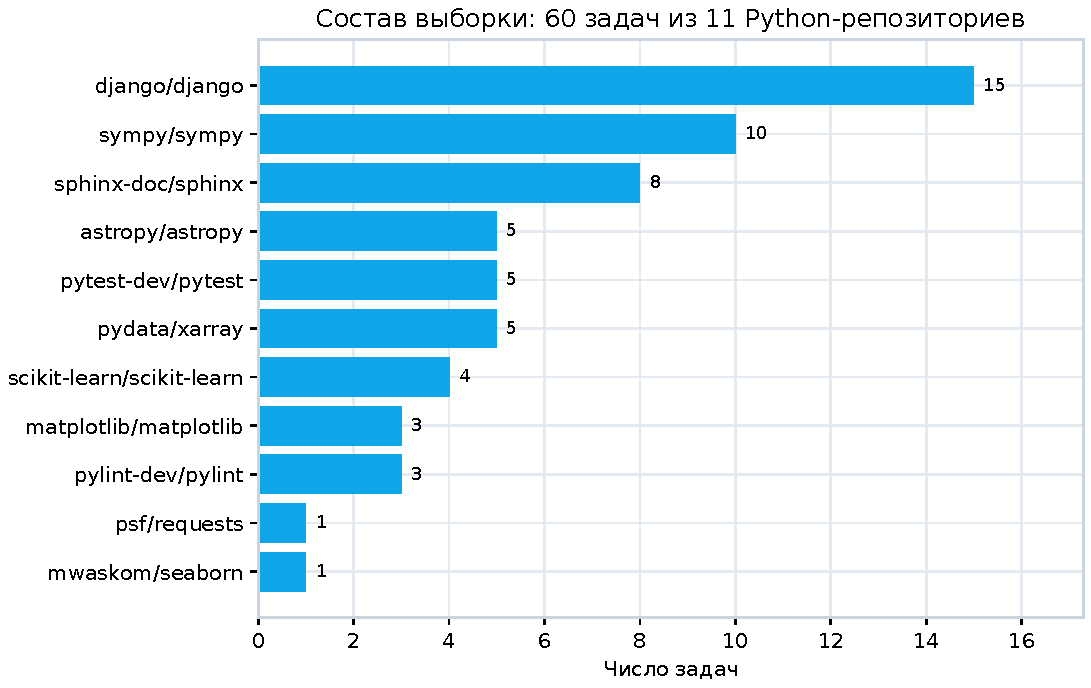
\includegraphics[width=0.9\textwidth]{fig_repository_distribution}
\caption{Число выбранных задач по репозиториям.}
\label{fig:repos}
\end{figure}

\subsection{Контролируемый кодовый контекст}

Для каждого instance использовался замороженный retrieval из набора
\code{princeton-nlp/SWE-bench\_bm25\_27K} ревизии
\code{d4667abc...} \cite{robertson2009bm25}. BM25 ранжирует документы по
совпадениям терминов с поправкой на частоту и длину документа; в данном
эксперименте ranking не пересчитывался после просмотра outcome. Из
официального артефакта извлекались только блоки \code{<code>}; legacy-поле
\code{text} не передавалось, поскольку содержало общий демонстрационный
patch.

Поиск дал от двух до восьми исходных файлов и от 71\,369 до 111\,192
символов на задачу; всего 245 файлов и 5\,691\,570 символов. Полученный
manifest использовался всеми методами. Независимое сопоставление каждого
файла с raw-содержимым нужного base commit дало 245/245 точных совпадений.
В матрице сохранялся SHA-256 контекста по каждой задаче. Поэтому различие
результата нельзя объяснить разным набором предоставленных файлов.

\begin{methodbox}[Граница утечки]
Generation runner мог читать только \code{instance\_id}, repository,
base commit, issue и извлечённые source-файлы. Gold patch, test patch,
\code{FAIL\_TO\_PASS}, \code{PASS\_TO\_PASS}, difficulty и selection rank
находились в отдельном sealed-файле, доступном evaluator только после
сохранения predictions.
\end{methodbox}

\section{Методы и экспериментальная матрица}

\subsection{Четыре метода основной серии}

\begin{table}[H]
\centering
\caption{Контролируемое различие между сравниваемыми методами.}
\label{tab:methods}
\begin{tabularx}{\textwidth}{@{}lXcc@{}}
\toprule
Метод & Последовательность & Вызовов & Задач\\
\midrule
Direct & немедленная генерация patch & 1 & 60\\
Один план & структурированный план, затем patch & 2 & 60\\
BVC & 4 роли, адаптивная критика, синтез, patch & 6 или 10 & 60\\
Полный совет & 4 роли, обязательная критика, синтез, patch & 10 & 60\\
\bottomrule
\end{tabularx}
\end{table}

Все методы используют одинаковую версию модели, temperature \(=0\), общий
контекст и одинаковую финальную patch-инструкцию. Один план и оба совета
передают patch-генератору совместимую структуру плана. Полный совет и BVC
имеют одинаковые роли, оси, синтезатор и максимальный бюджет. Следовательно,
адаптивность критики не смешана с наличием JSON-схемы либо самого
многоролевого разложения.

\subsection{Модель, лимиты и порядок исполнения}

\begin{table}[H]
\centering
\caption{Замороженная конфигурация generation runner.}
\label{tab:generation-config}
\begin{tabularx}{\textwidth}{@{}lX@{}}
\toprule
Параметр & Значение\\
\midrule
Провайдер / модель & Yandex Cloud AI Studio; requested
\code{deepseek-v4-flash}; returned \code{gpt://deepseek-v4-flash/latest}\\
Температура / seed & \(0\) / provider seed недоступен\\
Режим рассуждения & отдельный параметр thinking/non-thinking не передавался;
использован provider default, поле \code{reasoning\_content} сохранено\\
Prompt-версия & \code{main60-3.0.0}\\
Лимит роли & 4\,096 output-токенов\\
Лимит плана/синтеза & 4\,096 output-токенов\\
Лимит patch & 16\,384 output-токена; один repository-root unified diff\\
Порядок методов & детерминированная ротация
\code{bvc-main60-schedule-v1}\\
Primary guard & не более 1\,380 успешных вызовов, 1\,518 попыток и
45 млн токенов\\
\bottomrule
\end{tabularx}
\end{table}

Каждый API-ответ сохранялся целиком вместе с requested limit, usage,
finish reason, длительностью, prompt, plan/patch и SHA-256. Один primary
patch-вызов после повторяющихся transport-timeout был выполнен с read timeout
600 вместо 180 секунд; запрос не изменялся и завершился за 195,688 секунды.
Это отклонение касается транспорта и не меняет 60-задачные outcomes.
Доступность DeepSeek V4 Flash в Yandex Cloud подтверждается официальным
сообщением провайдера \cite{yandex2026deepseekv4}. Однако алиас
\code{latest} не является неизменяемым идентификатором весов: сохранённый
returned model URI точно документирует обслуженный запрос, но сам по себе не
гарантирует будущий запуск той же серверной ревизии.

\subsection{BVC как заранее включаемый режим}

Активационная политика BVC --- \code{human\_enabled\_before\_first\_edit}.
Сначала четыре независимые роли выдают решения по локализации причины,
стратегии исправления, зависимостям и тестовому покрытию. Затем вычисляются
\(D_{\mathrm{vote}}\) и \(D_{\mathrm{cov}}\). При превышении порогов
\(0{,}30\) и \(0{,}25\), либо при отсутствии оси с двумя валидными голосами,
выполняется один раунд критики. Эта схема продолжает проектную модель,
описанную в дипломе \cite{khalilov2026}, но в эксперименте реализована как
полностью исполняемый и хэшируемый протокол.
Пороги были зафиксированы как инженерные значения до просмотра outcomes;
они не настраивались на 60 тестовых задачах и не заявляются оптимальными.

\subsection{Три слоя эксперимента}

Основная матрица имеет размер
\[
60\ \text{задач}\times4\ \text{метода}=\NPrimaryRuns{}\ \text{строк}.
\]
Для 15 заранее выделенных задач выполнены два дополнительных повторения
трёх методов:
\[
15\times3\times2=\NRepeatRuns{}\ \text{дополнительных строк}.
\]
В сочетании с соответствующими 45 строками первой репетиции это даёт по
три outcome на задачу и метод. Наконец, для тех же 15 задач создан один
контролируемый разговорный paraphrase:
\[
15\times3=\NVibeRuns{}\ \text{строк}.
\]
Полный объём официальной оценки:
\[
\NPrimaryRuns+\NRepeatRuns+\NVibeRuns=\NAllRuns.
\]

\begin{figure}[H]
\centering
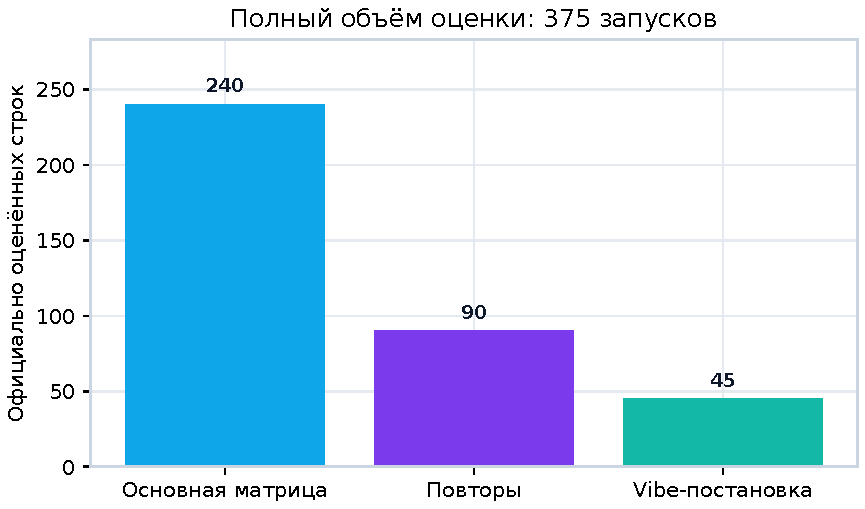
\includegraphics[width=0.82\textwidth]{fig_evaluation_layers}
\caption{Три слоя сохранённых официальных результатов.}
\label{fig:layers}
\end{figure}

\section{Цепочка аудируемости и воспроизводимости}

\begin{figure}[H]
\centering
\resizebox{0.98\textwidth}{!}{%
\begin{tikzpicture}[node distance=7mm and 8mm]
  \node[stage, text width=25mm] (snapshot) {Snapshot\\500 задач};
  \node[stage, right=of snapshot, text width=25mm] (selection) {Outcome-blind\\выбор 60};
  \node[stage, right=of selection, text width=25mm] (context) {Общий context\\manifest};
  \node[stage, right=of context, text width=25mm] (matrix) {Замороженная\\матрица};
  \node[stage, below=10mm of matrix, text width=25mm] (generation) {Call-артефакты\\и final JSON};
  \node[stage, left=of generation, text width=25mm] (eval) {Официальный\\evaluator};
  \node[stage, left=of eval, text width=25mm] (analysis) {Парный анализ\\и отчёт};
  \draw[flow] (snapshot) -- (selection);
  \draw[flow] (selection) -- (context);
  \draw[flow] (context) -- (matrix);
  \draw[flow] (matrix) -- (generation);
  \draw[flow] (generation) -- (eval);
  \draw[flow] (eval) -- (analysis);
  \node[note, below=2mm of generation] {hash prompt, content, patch};
  \node[note, below=2mm of eval] {apply + tests};
  \node[note, below=2mm of analysis] {JSON + SHA-256};
\end{tikzpicture}
}
\caption{Цепочка данных от snapshot до статистического вывода.}
\label{fig:lineage}
\end{figure}

\subsection{Заморозка до outcome}

До основной генерации фиксируются:
\begin{itemize}
  \item список задач и страты;
  \item контекстные manifests;
  \item prompts и их hash;
  \item version runner и модель;
  \item лимиты токенов, timeout и stop-rule;
  \item пороги gate;
  \item первичный contrast, bootstrap seed и правило множественных сравнений.
\end{itemize}
Это отделяет изменение исследовательского дизайна от исправления технической
ошибки исполнения. Любое допустимое транспортное отклонение сохраняется в
отдельном журнале и не удаляет уже наблюдавшиеся результаты.

Первичный contrast был заранее задан как BVC минус один план; margin
практически важной потери составлял \(-5\) \pp. Bootstrap seed
\code{bvc-main60-bootstrap-v1}, 10\,000 реплик и Holm-коррекция для двух
secondary-contrast также были зафиксированы до evaluation. Шесть других
реальных задач служили development-набором для проверки JSON, diff и harness;
они не входят ни в одну inferential-таблицу.

\subsection{Сохранение всех исходов}

Provider-successful вызов не гарантирует корректный diff. В основной серии
59/60 direct и 59/60 full-council patch были синтаксически разбираемы; BVC
и один план дали 60/60. Два некорректных результата сохранены и оценены как
сгенерированные outcomes. Результат не исключался по причине ошибки
применения patch, изменения тестового файла или нулевого успеха.

\subsection{Исполняемая оценка}

Evaluator последовательно проверял существование patch, синтаксическую
разбираемость, применимость к нужному checkout и прохождение тестов
\dataset{}. Только официальный статус \code{resolved=true} засчитывался как
успех. Правдоподобное объяснение модели без проходящих тестов не считалось
решением.

Использован официальный harness commit
\code{f7bbbb2ccdf479001d6467c9e34af59e44a840f9}. Patch применялся к
чистому base commit в контейнере; затем должны были пройти все требуемые
\code{FAIL\_TO\_PASS} и \code{PASS\_TO\_PASS} тесты. Официальные
per-instance reports были созданы для 18 BVC, 14 direct, 18 full-council и
20 single-plan predictions. Для неприменимых непустых patches официальный
лог содержал буквальный статус \code{Patch Apply Failed}; такие строки
сохранялись как \code{resolved=false}. Один пустой direct-patch и один
пустой full-council patch также остались неуспехами. Для бинарной метрики
отсутствие report по любой другой причине также кодировалось как 0 и отдельно
помечалось как инфраструктурный случай, а не исключалось из знаменателя.

\begin{table}[H]
\centering
\caption{Переход от применимого patch к официально решённой задаче.}
\label{tab:apply-resolve}
\begin{tabular}{@{}lrrr@{}}
\toprule
Метод & Применимо & Решено & Решено среди применимых\\
\midrule
Direct & 14 & 4 & 28,6\%\\
Один план & 20 & 7 & 35,0\%\\
BVC & 18 & 5 & 27,8\%\\
Полный совет & 18 & 6 & 33,3\%\\
\bottomrule
\end{tabular}
\end{table}

Условная доля «решено среди применимых» описывает воронку после генерации и
не является отдельным причинным эффектом качества плана: применимость patch
сама зависит от метода. Таблица нужна для локализации потерь между синтаксисом,
применением и тестами, а не для post-hoc ранжирования алгоритмов.

Шесть primary-patch изменяли тестовые файлы. Все шесть официально неуспешны
и сохранены, поэтому test-edit не создаёт ни одного функционального успеха
и не объясняет сравнительный результат.

\begin{figure}[H]
\centering
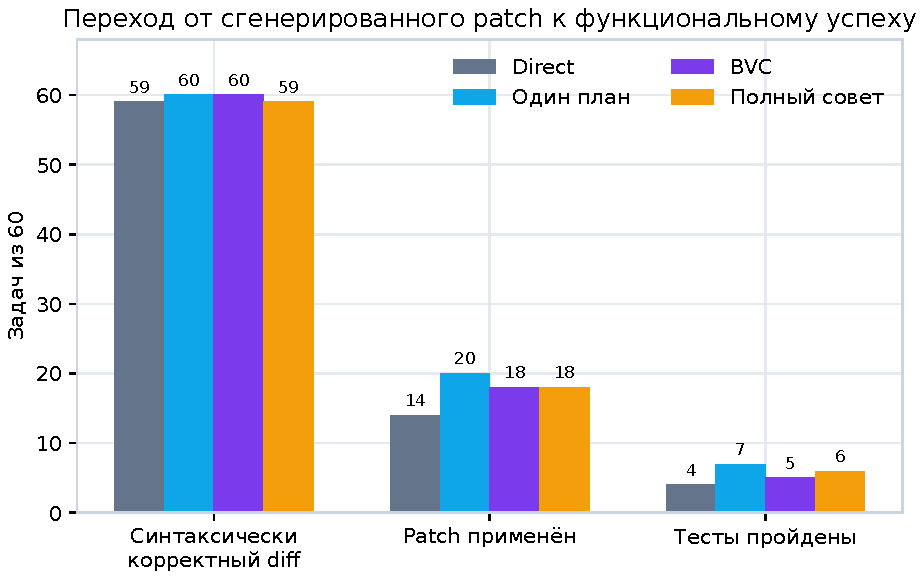
\includegraphics[width=0.92\textwidth]{fig_evaluation_funnel}
\caption{Число результатов на трёх стадиях исполняемой проверки.}
\label{fig:funnel}
\end{figure}

\section{Проверки целостности}

\subsection{Полнота матриц}

\begin{table}[H]
\centering
\caption{Автоматические проверки трёх экспериментальных слоёв.}
\label{tab:integrity}
\begin{tabular}{@{}lrrrrl@{}}
\toprule
Слой & Ожидалось & Получено & Пропуски & Дубликаты & Статус\\
\midrule
Основная матрица & 240 & 240 & 0 & 0 & passed\\
Дополнительные повторы & 90 & 90 & 0 & 0 & passed\\
Разговорная постановка & 45 & 45 & 0 & 0 & passed\\
\midrule
Всего & 375 & 375 & 0 & 0 & complete\\
\bottomrule
\end{tabular}
\end{table}

Во всех трёх слоях число несовпадений hash prompt равно нулю; число
несовпадений hash content также равно нулю. В основной серии сохранено
1\,268 call-артефактов, из них 1\,255 успешных вызовов и 13 неуспешных
попыток. В принятых финальных маршрутах 240 строк содержится 1\,252 успешных
вызова: \(60+120+472+600\) для direct, одного плана, BVC и полного совета.
Оставшиеся три успешных артефакта --- плановые вызовы из вытесненных попыток
1--3 для \code{sympy\_\_sympy-12489}; соответствующие patch-вызовы
прерывались транспортно, а принятый результат получен в попытке 4. Эти три
вызова входят в аудит фактического расхода, но не в число вызовов финального
маршрута. Аудит не подменяет функциональные тесты, но подтверждает, что
итоговая таблица относится к замороженным inputs. Совпадение hash проверяет
буквальное содержимое сохранённых prompt и context; оно не доказывает
семантическую корректность произвольной metadata-метки.

\subsection{Контроль расхода}

Общий cost-guard по всем созданным артефактам зарегистрировал 1\,848
успешных вызовов, \num{\AllTokens} токенов и \num{\AllCost} руб.
расчётной стоимости при stop-пороге \num{\CostCap} руб. Здесь объём шире
\NAllRuns{} официальных строк: он включает технические и незавершённые
попытки, которые нужны для честного учёта фактического расхода.

\section{Статистический план}

\subsection{Парная разность долей}

Пусть \(Y_{im}\in\{0,1\}\) --- официальный outcome задачи \(i\) для метода
\(m\). Для двух методов \(A\) и \(B\)
\[
\widehat{\Delta}_{A-B}
=\frac{1}{n}\sum_{i=1}^{n}(Y_{iA}-Y_{iB}).
\]
Такое определение сохраняет task-level pairing. Например, одинаковый успех
обоих методов даёт нулевой вклад, а успех только BVC --- \(+1/n\).

\subsection{Точный критерий Мак-Немара}

Пусть \(b\) --- число задач, решённых только \(A\), а \(c\) --- только \(B\).
При нулевой гипотезе направления \(b+c\) дискордантных пар равновероятны.
Двустороннее точное значение:
\[
p_{\mathrm{exact}}
=\min\!\left(
1,\;
2\sum_{k=0}^{\min(b,c)}
\binom{b+c}{k}2^{-(b+c)}
\right).
\]
Критерий использует именно те задачи, на которых методы различились
\cite{mcnemar1947}.

\subsection{Стратифицированный paired bootstrap}

Для каждой из трёх страт сложности задачи повторно выбираются с возвращением
внутри своей страты; затем страты объединяются с исходными размерами
30, 27 и 3. Для каждой из 10\,000 детерминированных реплик вычисляется
\(\widehat{\Delta}^{\ast}\). Интервал --- 2,5-й и 97,5-й процентили.
Так одновременно сохраняются pairing и состав по сложности
\cite{efron1993bootstrap}.

Внутри одной bootstrap-реплики выбирается именно \emph{задача}, а не
отдельный outcome метода: вся пара \((Y_{iA},Y_{iB})\) переносится вместе.
Иначе корреляция методов на одной задаче была бы разрушена, а интервал отвечал
бы на другой, непарный вопрос.

\subsection{Интервалы отдельных долей и множественные сравнения}

Для визуализации каждой доли используется Wilson-интервал
\cite{wilson1927}. Он не заменяет парный анализ. Сравнение BVC с одним
планом объявлено первичным. Два secondary-contrast --- с direct и полным
советом --- корректируются методом Holm \cite{holm1979}. Ни одно значение
\(p\) не интерпретируется отдельно от числа дискордантных пар и интервала
эффекта.

Для \(x\) успехов из \(n\), \(\widehat p=x/n\) и квантиля
\(z=1{,}96\) центр Wilson-интервала равен
\[
\widetilde p=
\frac{\widehat p+z^2/(2n)}{1+z^2/n},
\]
а полуширина ---
\[
h=
\frac{z}{1+z^2/n}
\sqrt{\frac{\widehat p(1-\widehat p)}{n}+\frac{z^2}{4n^2}}.
\]
Показывается \([\widetilde p-h;\widetilde p+h]\). Для Holm два
secondary-\(p\) сортируются; меньшее сравнивается с \(\alpha/2\), следующее
--- с \(\alpha\). В текущих данных оба raw-\(p\) равны 1, поэтому
adjusted-\(p\) также равны 1.

\section{Результаты основной матрицы}

\begin{table}[H]
\centering
\caption{Функциональный результат и 95\% Wilson-интервал.}
\label{tab:outcomes}
\begin{tabular}{@{}lrrr@{}}
\toprule
Метод & Решено & Доля & 95\% Wilson CI\\
\midrule
Direct & \DirectResolved/60 & \DirectRate\% & [\DirectWilsonLow; \DirectWilsonHigh]\%\\
Один план & \SingleResolved/60 & \SingleRate\% & [\SingleWilsonLow; \SingleWilsonHigh]\%\\
BVC & \BVCResolved/60 & \BVCRate\% & [\BVCWilsonLow; \BVCWilsonHigh]\%\\
Полный совет & \FixedResolved/60 & \FixedRate\% & [\FixedWilsonLow; \FixedWilsonHigh]\%\\
\bottomrule
\end{tabular}
\end{table}

\begin{figure}[H]
\centering
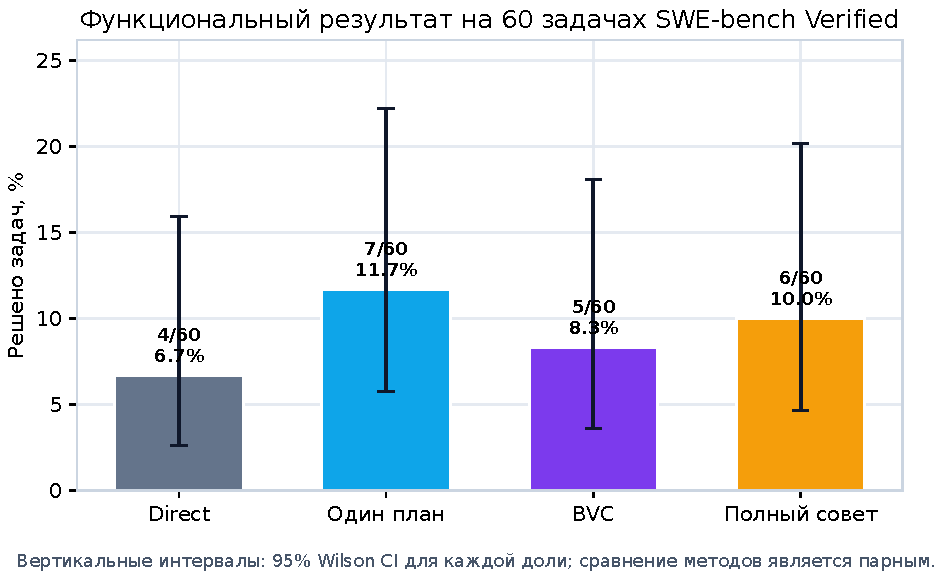
\includegraphics[width=0.9\textwidth]{fig_success_wilson}
\caption{Доли решённых задач; интервалы отдельных долей показаны для масштаба неопределённости.}
\label{fig:success}
\end{figure}

\begin{table}[H]
\centering
\caption{Парные сравнения BVC с тремя режимами.}
\label{tab:paired}
\begin{tabularx}{\textwidth}{@{}Xrrrrr@{}}
\toprule
Contrast & BVC-only & Baseline-only & Разность, \pp & 95\% bootstrap & \(p\)\\
\midrule
BVC --- один план (primary) & 1 & 3 & \(-3{,}3\) & \([-10{,}0;+3{,}3]\) & 0,625\\
BVC --- direct & 1 & 0 & \(+1{,}7\) & \([0{,}0;+5{,}0]\) & 1,000\\
BVC --- полный совет & 0 & 1 & \(-1{,}7\) & \([-5{,}0;0{,}0]\) & 1,000\\
\bottomrule
\end{tabularx}
\end{table}

\begin{figure}[H]
\centering
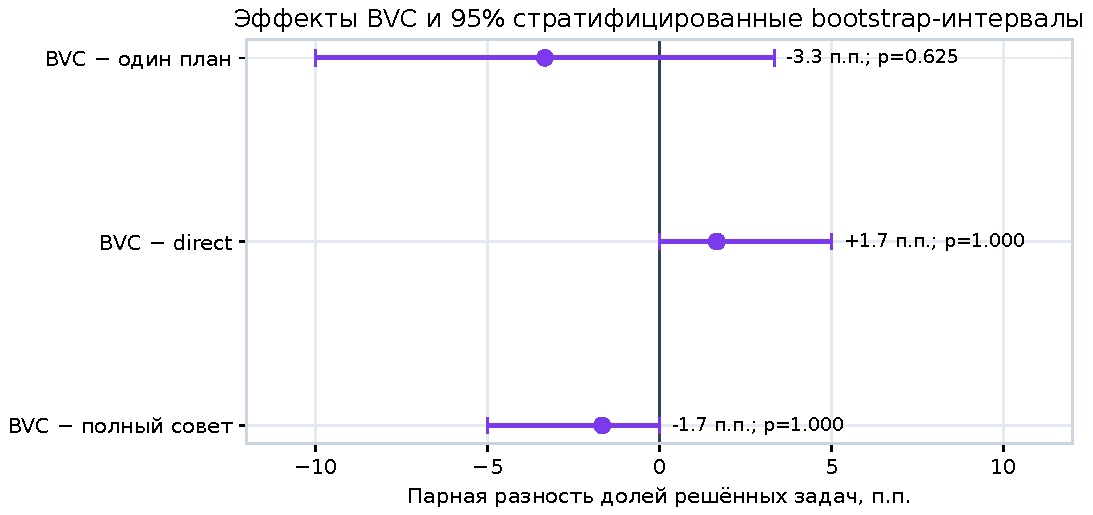
\includegraphics[width=0.9\textwidth]{fig_paired_effects}
\caption{Точечные оценки и замороженные bootstrap-интервалы парных эффектов.}
\label{fig:effects}
\end{figure}

Для двух secondary-contrast одна клетка дискордантности пуста. Поэтому
процентильные интервалы вырождены по знаку: каждая bootstrap-реплика BVC--direct
неотрицательна, а BVC--полный совет неположительна. Границы 0,0 в интервалах
\([0{,}0;+5{,}0]\) и \([-5{,}0;0{,}0]\) отражают структуру этой матрицы,
а не являются самостоятельным подтверждением знака истинного эффекта.

Основная заранее заявленная гипотеза преимущества BVC над одним планом
не поддержана: наблюдаемая разность отрицательна, интервал включает ноль,
точный тест не значим. С direct получен положительный описательный сигнал:
пять решений против четырёх, причём одна задача решена только BVC. Но
единственная дискордантная пара даёт \(p=1{,}0\); это основание для
следующего эксперимента, а не доказательство превосходства.
Заранее заданная неухудшаемость с margin \(-5\) \pp{} также не установлена:
нижняя граница 95\% интервала первичного эффекта равна \(-10\) \pp.

\section{Ресурсные метрики}

\begin{table}[H]
\centering
\caption{Фактическая эффективность в основной матрице.}
\label{tab:cost}
\begin{tabular}{@{}lrrrrr@{}}
\toprule
Метод & Вызовы & Токены & Цена, руб. & Руб./задачу & Руб./решённую\\
\midrule
Direct & \num{\DirectCalls} & \num{\DirectTokens} & \num{\DirectCost} &
\num{\DirectCostTask} & \num{\DirectCostResolved}\\
Один план & \num{\SingleCalls} & \num{\SingleTokens} & \num{\SingleCost} &
\num{\SingleCostTask} & \num{\SingleCostResolved}\\
BVC & \num{\BVCCalls} & \num{\BVCTokens} & \num{\BVCCost} &
\num{\BVCCostTask} & \num{\BVCCostResolved}\\
Полный совет & \num{\FixedCalls} & \num{\FixedTokens} & \num{\FixedCost} &
\num{\FixedCostTask} & \num{\FixedCostResolved}\\
\bottomrule
\end{tabular}
\end{table}

Наиболее корректная ресурсная пара --- BVC и полный совет, потому что они
совпадают по ролям и максимальному маршруту. BVC сократил вызовы на 21,3\%,
токены на 22,2\% и стоимость на 23,5\%. На карте стоимости и качества
точки показаны без попытки объединить рубли и success rate в произвольный
единый score.

Парный расширенный расчёт по каждой задаче даёт среднюю экономию
\num{\CallsSavedTaskMean} вызова, \num{\TokensSavedTask} токенов и
\num{\CostSavedTask} руб. на задачу. Соответствующие 95\%
bootstrap-интервалы равны
\([\num{\CallsSavedTaskMeanLow};\num{\CallsSavedTaskMeanHigh}]\) вызова,
\([\num{\TokensSavedTaskMeanLow};\num{\TokensSavedTaskMeanHigh}]\) токенов
и \([\num{\CostSavedTaskMeanLow};\num{\CostSavedTaskMeanHigh}]\) руб.
Эти интервалы относятся к среднему ресурсному эффекту на замороженной
смеси страт и добавлены как прозрачный
описательный анализ; primary inference по качеству от них не меняется.

\begin{figure}[H]
\centering
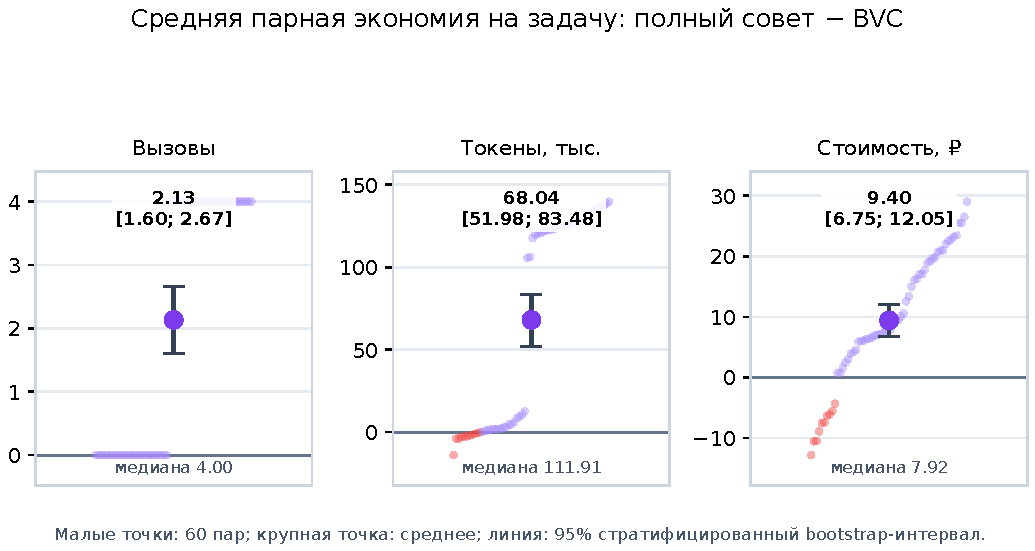
\includegraphics[width=0.9\textwidth]{fig_resource_paired_effects}
\caption{Средняя парная экономия полного совета относительно BVC;
95\% интервалы получены 10\,000-кратным bootstrap внутри страт.}
\label{fig:resource-paired}
\end{figure}

\begin{figure}[H]
\centering
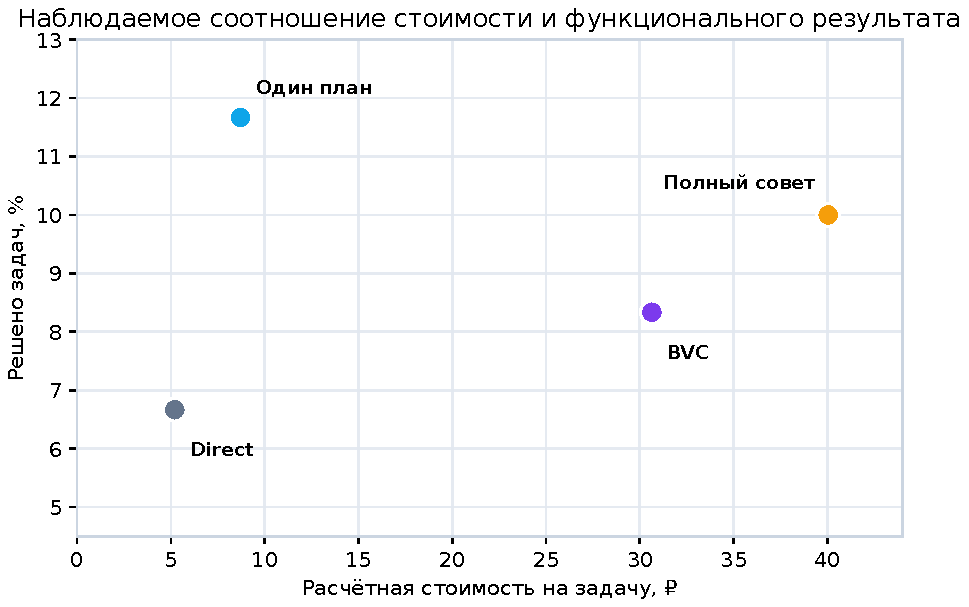
\includegraphics[width=0.88\textwidth]{fig_cost_quality}
\caption{Наблюдаемая стоимость на задачу и функциональный результат.}
\label{fig:cost-quality}
\end{figure}

\section{Повторяемость}

Temperature \(=0\) не делает полный pipeline детерминированным: возможны
различия провайдера, окружения и генерации. Для 15 задач сравнивались три
формальных исхода каждого из direct, одного плана и BVC.

\begin{table}[H]
\centering
\caption{Функциональный outcome в трёх повторах.}
\label{tab:repeat}
\begin{tabular}{@{}lrrrrr@{}}
\toprule
Метод & Повтор 1 & Повтор 2 & Повтор 3 & Все три совпали & Попарное согласие\\
\midrule
Direct & 0/15 & 2/15 & 1/15 & 13/15 & 91,1\%\\
Один план & 1/15 & 1/15 & 2/15 & 13/15 & 91,1\%\\
BVC & 0/15 & 2/15 & 0/15 & 13/15 & 91,1\%\\
\bottomrule
\end{tabular}
\end{table}

\begin{figure}[H]
\centering
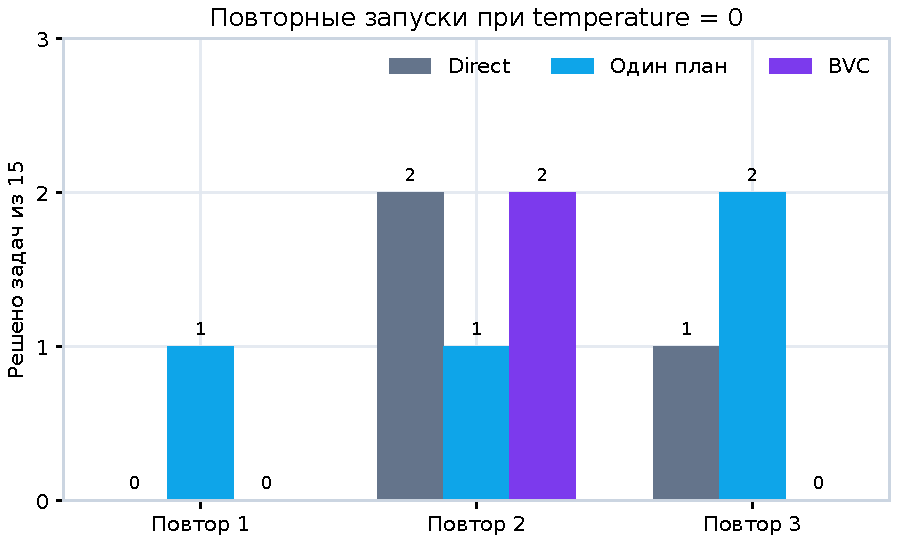
\includegraphics[width=0.88\textwidth]{fig_repeatability}
\caption{Число решённых задач в каждом повторе при temperature \(=0\).}
\label{fig:repeat}
\end{figure}

Для каждого метода все три бинарных исхода совпали на 86,7\% задач, среднее
попарное согласие равно 91,1\%. Эти значения характеризуют наблюдаемый
pipeline и не подменяют primary-оценку на 60 задачах. Majority outcome BVC
равен 0/15, одного плана --- 2/15; точный парный \(p=0{,}5\).

Этот вспомогательный 15-задачный слой не является прямой оценкой дисперсии
60-задачного contrast и не аннулирует замороженную основную матрицу. Однако
колебание числа успехов от 0 до 2 из 15 при неизменном nominal setup
показывает, что одиночные различия в одну--две задачи нельзя считать
устойчивым свидетельством качества. Для такой оценки нужны как минимум три
и более запуска каждого метода на всей сравниваемой выборке либо отдельная
модель вероятности успеха на instance.

В repeat-слое транспортное окно также временно увеличивалось до 600 секунд
после повторных timeout. Два поздних успешных API-ответа заняли более
180 секунд. Все затронутые задачи официально остались unresolved, поэтому
ни один наблюдаемый успех или majority-success не создан расширенным
timeout; контрфактический ответ при строгом 180-секундном обрыве неизвестен.

\section{Устойчивость к разговорной формулировке}

Для тех же 15 instances фактическое требование и кодовый контекст сохранены,
но формальная инструкция переформулирована разговорно. Это контролируемая
проверка одного paraphrase, а не обобщение на весь класс vibe coding.

Финальный файл разговорных входов имеет отдельный SHA-256; все 15 текстов
прошли model-based fidelity check и последующее ручное сопоставление
acceptance criteria. В per-row metadata по технической причине осталось
\code{prompt\_variant=formal}, однако это поле не участвовало в построении
prompt. Сохранённые API-prompts содержат именно разговорный текст. Регенерация
ради косметической метки не выполнялась, чтобы не выбирать новый outcome при
недоступном provider seed.

\begin{table}[H]
\centering
\caption{Формальная и разговорная постановки.}
\label{tab:vibe}
\begin{tabular}{@{}lrrrr@{}}
\toprule
Метод & Формально & Разговорно & Согласие по задачам & \(p_{\mathrm{McNemar}}\)\\
\midrule
Direct & 0/15 & 2/15 & 86,7\% & 0,5\\
Один план & 1/15 & 1/15 & 100,0\% & 1,0\\
BVC & 0/15 & 1/15 & 93,3\% & 1,0\\
\bottomrule
\end{tabular}
\end{table}

\begin{figure}[H]
\centering
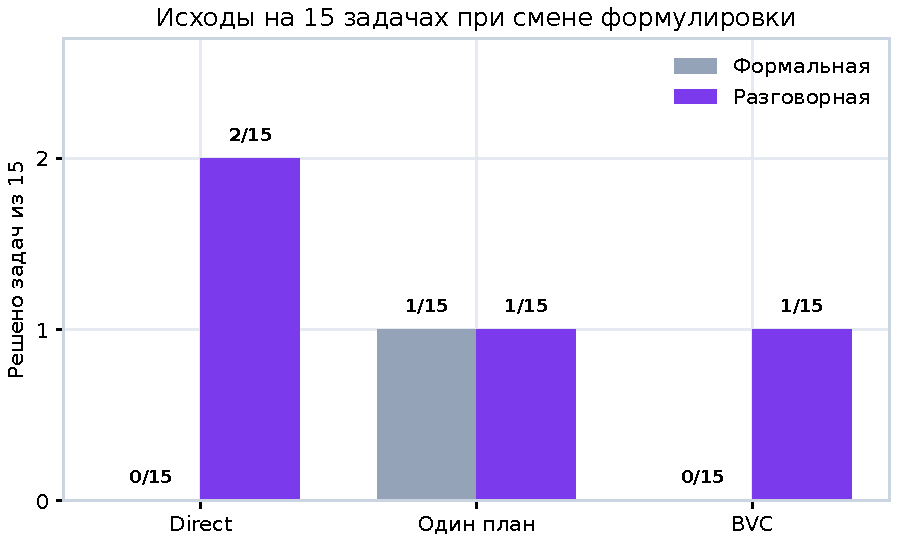
\includegraphics[width=0.88\textwidth]{fig_formal_vibe}
\caption{Исходы методов после контролируемой смены стиля запроса.}
\label{fig:vibe}
\end{figure}

BVC дал один успех в разговорной серии и сохранил одинаковый бинарный
outcome на 14/15 задачах. Это документированный исход одного paraphrase, но
не доказательство общей устойчивости: изменения direct и BVC находятся в
пределах колебания 0--2 успеха, уже наблюдавшегося в формальных повторах.

\section{Машиночитаемый пакет и доступность результатов}

Ключевые входы анализа имеют следующие SHA-256:

\begin{methodbox}[Проверяемые источники]
\begin{description}[style=nextline]
  \item[Основные 240 строк]
  \path{02b8fbcc05512aac41bae0fd4d0013912ef0b2d14436eb74d94f72bfae6892e3}
  \item[90 дополнительных повторов]
  \path{124e689cdb45cb79a550179c858cfc70a9a612b93d93101dd3abf309f8197220}
  \item[45 разговорных запусков]
  \path{65c4c6992fbbc5a658828f5c672f4c6016d690997587f2bd6d1ab38cc3817d37}
  \item[Замороженный robustness-протокол]
  \path{6aa01afcdcebd095b264f58865b5fb6f173bb93bf2b5a136110845eacddf3371}
\end{description}
\end{methodbox}

Сопроводительный пакет содержит исходные JSONL основной, repeat- и
разговорной серий, результаты integrity-проверок, frozen protocols, manifests,
скрипты анализа и исходники статей. На момент подготовки рукописи пакету не
присвоены публичный DOI или постоянный URL. Поэтому приведённые SHA-256
позволяют проверить уже полученную копию, но сами по себе не обеспечивают к
ней доступ. Точный статус результата --- аудируемый и пересчитываемый из
сопроводительного пакета; независимая публичная воспроизводимость потребует
публикации архива в постоянном репозитории.

Воспроизводимость здесь означает возможность проверить неизменность входов,
повторно выполнить агрегацию и увидеть все строки, включая неуспехи. Она не
означает гарантированного воспроизведения тех же модельных токенов внешним
провайдером в будущем.

\section{Связь с дипломом и практическая ценность}

Диплом \cite{khalilov2026} задаёт продуктовую архитектуру Xynapse и идею
ограниченного многоролевого анализа. Настоящий контур добавляет к ней
исследовательский слой: замороженную выборку, baselines, официальный
evaluator, парную статистику и ресурсный аудит. Поэтому в последующих
публикациях диплом корректно цитируется как источник архитектуры и метода,
а числовые claims ссылаются на экспериментальные JSONL и анализ.

Контур можно повторно использовать при замене модели. Для корректного
сравнения достаточно создать новую матрицу с теми же task IDs и context
hashes, сохранить полный набор финальных строк и выполнить тот же анализ.
Изменение тарифа не требует повторной генерации: стоимость пересчитывается
из трёх сохранённых категорий токенов.

Особенно важна эта воспроизводимость для продукта: при обновлении модели
команда может не спорить по отдельным красивым примерам, а провести тот же
парный тест и увидеть, изменились ли функциональный outcome, решение gate и
цена маршрута. В результате BVC получает накопительную экспериментальную
историю, а каждое следующее улучшение становится сопоставимым с предыдущим.

\section{Границы вывода}

Выборка содержит 60 задач и одну основную модель; интервалы success rate
остаются широкими. Не проверен equal-budget best-of-\(k\) или self-consistency
baseline, поэтому эксперимент изолирует адаптивный gate относительно его
собственной неадаптивной версии, но не доказывает оптимальность многоролевого
расходования бюджета. Контекст ограничен BM25-выборкой файлов, patch создаётся
одним вызовом без инструментов, запуска тестов и обратной связи, тогда как
современные coding workflows используют поиск и итерации
\cite{xia2024agentless,yang2024sweagent}. Разговорная серия использует один
paraphrase и 15 задач. Повторы оценивают бинарный outcome, а не семантическое
сходство планов. Алиас модели \code{latest} и отсутствие provider seed
дополнительно ограничивают точное повторение генерации.
После проведения эксперимента опубликован аудит, согласно которому
\dataset{} больше не подходит для измерения актуальной frontier coding
capability из-за остаточных дефектов тестов и контаминации
\cite{openai2026verifiedlimits}. Поэтому настоящая работа не трактует
8,3\% или 11,7\% как абсолютную оценку способности модели. Парный дизайн
остаётся проверкой четырёх workflows на одной фиксированной матрице и одном
evaluator, но вывод ограничен именно этим тестом. Эти границы точно определяют
масштаб утверждений и не позволяют смешать описательный сигнал с
подтверждённой гипотезой.

Три сопроводительные статьи используют одну и ту же основную матрицу
240 запусков, а не три независимых эксперимента. Они разделяют вопросы:
адаптивный бюджет, аудируемый контур и чувствительность к стилю запроса.
Совпадение исходных данных между статьями поэтому раскрывается явно и не
может интерпретироваться как независимая репликация.

\section{Заключение}

Главный результат статьи --- BVC получил полноценный доказательный контур, а
не только архитектурное описание. Создана матрица из \NAllRuns{} официально оценённых
строк: 240 основных, 90 дополнительных повторов и 45 разговорных запусков.
Целостность всех матриц подтверждена, несовпадения prompt/content hash
отсутствуют. Основная гипотеза преимущества BVC над одним планом не
поддержана; положительный сигнал против direct равен одной дополнительной
решённой задаче и не является статистически значимым; неухудшаемость
относительно одного плана также не установлена. Одновременно
адаптивная экономия относительно полного совета измерена напрямую.
Тем самым проект Xynapse/BVC, исходно описанный в дипломе
\cite{khalilov2026}, получил проверяемую экспериментальную основу, пригодную
для следующих моделей, выборок и статей. С инженерной точки зрения это сильное
преимущество метода: его поведение, цена и границы качества можно не
предполагать, а последовательно измерять и улучшать.

\section*{Декларации}

Финансирование и конфликт интересов отсутствуют. LLM использовались для
генерации экспериментальных ответов и языковой редакции; функциональный
outcome определён официальным исполняемым evaluator, а все числовые значения
статей вычислены из сохранённых JSON/JSONL. Диплом \cite{khalilov2026}
цитируется как источник архитектуры Xynapse/BVC, но не как источник
экспериментальных результатов настоящей работы.

\printbibliography[title={Литература}]
\end{document}
